\chapter{Background}
This chapter provides a summary of all of the project's topics. Starting with the main one, what is a VPN and specifically how WireGuard works, followed by an overview of the operating system used, FreeRTOS. There is also a description of the Lightweight IP Stack and of the board used for the project.
\section{VPN}
A VPN is a Virtual Private Network that guarantees confidentiality, integrity and authentication, through a secure communication channel (VPN tunnel).\\
With this service all the Internet traffic is encrypted and the user is able to protect his online identity, in fact it allows to mask the IP (Internet Protocol) and so the real position.\\
The term \emph{Virtual} means that the devices in this network can be located anywhere in the world, and it is not necessary that they are all under the same local network.

\subsection{VPN classification}
There are two types of VPN:
\begin{itemize}
    \item Remote Access VPN: it allows the user to connect to a server on a private network. 
    \item Site-To-Site VPN: it refers to a connection set up between multiple networks which allows secure routing and communication.\\
        Considering the level of reliability and safety, this type of VPN can also be divided in:
        \begin{itemize}
            \item Trusted: Internet Service Provider (ISP) guarantees the data protection.
            \item Secure: it uses encryption protocols to guarantees the creation of a secure tunnel between the private network nodes. In this way the data inside the tunnel are protected against possible external attacks.
            \item Hybrid: it is a mix of a secure VPN and a trusted one.
        \end{itemize}
\end{itemize}

\subsection{How VPN works}
A VPN uses a tunnelling mechanism, that allows the creation of a secure channel between two remote entities.
The data packets sent in this channel are encapsulated by the tunneling protocol and encrypted.\\
In this way the data are protected against possible external attacks and all the traffic is \emph{invisible} in the public network, because the user ip is masked so formally he is not receiving or sending anything.
In the image \ref{fig:vpnTunnel} it can be seen the logical tunnel that protects the data packets.
\begin{figure}[H]
    \vspace{0.5cm}
    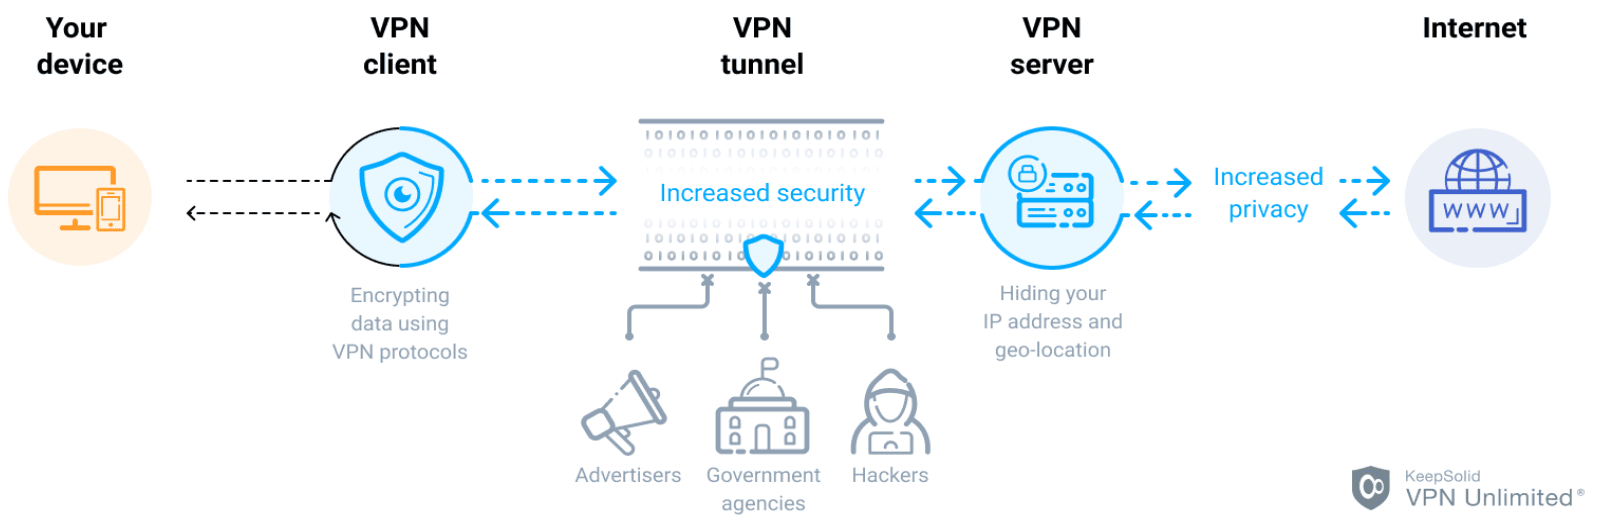
\includegraphics[width=\textwidth, scale=0.25]{images/vpnTunnel.png}
    \caption{VPN tunnelling}
    \label{fig:vpnTunnel} % This is the image label, with which you can refer to the image in any document location.

\end{figure}


\section{WireGuard}
Among all the available VPN, Wireguard \cite{WireGuard} was the one chosen for this project.\\
It is an extremely simple modern VPN which uses state-of-the-art cryptography and it is also Free and Open Source. 
WireGuard is a secure VPN, so through tunnelling, it securely encapsulates IP packets over UDP.\\
How it works is simple: it simply gives a virtual interface which can then be administered using the standard \texttt{ip(8)} and \texttt{ifconfig(8)} utilities. After configuring the interface with a private key and the various public keys of peers with whom it will communicate
securely, the tunnel simply works.

\subsection{How WireGuard works}
The fundamental principle of a secure VPN is an association between peers and the IP addresses each is allowed
to use as source IPs. In WireGuard, peers are identified strictly by their public key, so there is a simple association mapping between public keys and a set of allowed IP addresses.\\
In the following there is an example of a possible crypto key routing table \ref{fig:WGinterface}:

\begin{figure}[H]
    \vspace{0.5cm}
    \includegraphics[width=\textwidth, scale=0.25]{images/wgInterface\_example.png}
    \caption{Cryptokey routing table for a WireGuard Network Interface}
    \label{fig:WGinterface} % This is the image label, with which you can refer to the image in any document location.
\end{figure}

The interface itself has a private key and a UDP port for listening, followed by a list of peers. Each peer is identified by its public key and each has a list of allowed source IPs.\\
It is important that peers are able to send encrypted WireGuard UDP packets to each other at particular Internet endpoints. Each peer in the cryptokey routing table may optionally pre-specify a known external IP address and UDP port of that peer’s endpoint (adding in \ref{fig:WGinterface} an Internet Endpoint in the form IP:UDPport).
It is optional because if it is not specified and WireGuard receives a correctly authenticated packet from a peer, it will use the outer external source IP
address for determining the endpoint.\\
When an outgoing packet is being transmitted on a WireGuard network interface, called wg0, this table is consulted to determine which public key to use for encryption.\\
Using \ref{fig:WGinterface}, when receiving and sending a packet on interface wg0 there will be the following flow:\\
A packet is locally generated and is ready to be transmitted on the outgoing interface wg0:
\begin{enumerate}
    \item The plaintext packet reaches the WireGuard interface, wg0.
    \item The destination IP address of the packet, 192.168.87.21, is inspected, which matches the peer TrMv...WXX0
    \item The symmetric sending encryption key and nonce counter of the secure session associated with peer TrMv...WXX0 are used to encrypt the plaintext packet using ChaCha20Poly1305.
    \item A header containing various fields is prepended to the now encrypted packet.
    \item This header and encrypted packet, together, are sent as a UDP packet to the Internet UDP/IP endpoint associated with peer TrMv...WXX0, resulting in an outer UDP/IP packet containing as its payload a header and encrypted inner-packet. 
\end{enumerate}
A UDP/IP packet reaches UDP port 41414 of the host, which is the listening UDP port of interface wg0:
\begin{enumerate}
    \item A UDP/IP packet containing a particular header and an encrypted payload is received on the correct port.
    \item Using the header WireGuard determines that it is associated with peer TrMv...WXX0’s secure session, checks the validity of the message counter, and attempts to authenticate and decrypt it using the secure session’s receiving symmetric key. If it cannot determine a peer or if authentication fails, the packet is dropped.
    \item Since the packet has authenticated correctly, the source IP of the outer UDP/IP packet is used to update the endpoint for peer TrMv...WXX0.
    \item Once the packet payload is decrypted, the interface has a plaintext packet. If this is not an IP packet, it is dropped. Otherwise, WireGuard checks to see if the source IP address of the plaintext inner-packet routes correspondingly in the crypto key routing table.
    \item If the plaintext packet has not been dropped, it is inserted into the receive queue of the wg0 interface.
\end{enumerate}

\textbf{NOTE}: This explanation part is provided as it reported on the official WireGuard whitepaper \cite{WireGuard}. 

\subsection{Cryptographic Algorithms}\label{sec:WGAlgo}
WireGuard uses state-of-the-art cryptography. Among all the possible algorithms, the ones used in this project are:
\begin{itemize}
    \item BLAKE2S : it is a cryptographic hash function optimized for 8 to 32-bit platforms and it produces digests of any size between 8 bits and 256 bits.
    \item X25519 : it is an elliptic curve DiffieHellman key exchange using Curve25519, which is an elliptic curve offering 128 bits of security (256 bits of key size). It allows two parties to jointly agree on a shared secret using a non-secure channel.
    \item CHACHA20-POLY1305 : it is an Authenticated Encryption with Additional Data (AEAD) algorithm. It combines the ChaCha20 stream cipher (whose input includes a 256-bit key, a 32-bit counter, a 96-bit nonce and plain text) with the Poly1305 message authentication code.
\end{itemize}
\subsubsection{Authenticated Encryption with Additional Data Algorithm (AEAD)}
It is an algorithm that guarantees both confidentiality (through encryption) as well as integrity and authenticity of data.\\
Encryption only provides confidentiality, but the message sent is not protected against modification. So, additional data must be transmitted along with the message to authenticate it. For AEAD this operation takes the form of a MAC (Message Authentication Code).\\
Keyed hash functions are commonly used to generate MACs.


%simone
\section{FreeRTOS}\label{freertos}
FreeRTOS is a real-time OS which is based on a simple kernel, and it is widely used in many embedded systems applications. It is owned and developed by Real Time Engineers Ltd. 
The application could be organized in different threads that could be executed on different type of processors and the execution order is computed by the kernel basing on the priority of the different tasks, which is assigned by the application designer. Usually, the tasks with more strict time requirements have the higher priority with respect to the one more time tolerant. 

\subsection{FreeRTOS distribution}\label{freertosdistribution}
FreeRTOS could be seen as a library composed of many C source files that provides multi-tasking capabilities. Compiling these files with the target application make it able to reach the FreeRTOS API. In order to simplify the development with this library, many different demo projects, that are preconfigured to compile the correct source files, are inserted in the FreeRTOS released folder.\\
FreeRTOS is configured by the FreeRTOSConfig.h header which is used to setup the OS to fit the target application. It contains different configuration in order to set parameters like, for example, the scheduling algorithm. This file must be located in a directory that is part of the application that has been built. 
The official distribution is given with first and second directory as can be seen in figure \ref{fig:freeRTOSFolder} 

\begin{figure}[H]
\vspace{0.4cm}
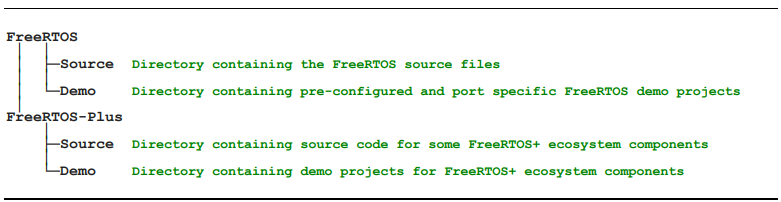
\includegraphics[width=\textwidth]{images/freeRTOS_folder.png}
\caption{FreeRTOS directory tree.}
\label{fig:freeRTOSFolder} % This is the image label, with which you can refer to the image in any document location.
\end{figure}

For more details on FreeRTOS you can check the official site (\cite{FreeRTOSPage}) and the guide (\cite{FreeRTOSGuide})









%Lorenzo
\section{The Lightweight IP Stack - LwIP}\label{lwip}
The Lightweight IP Stack (LwIP) is a very small complete implementation of many network protocols, most importantly it provides everything that is needed for a TCP connection (IP, ICMP, ARP), it is predisposed for some useful protocols like NTP, and PPP.
\\LwIP is built to be easy to port to new platform, which is needed for any hardware change.\\
Only a few files have to be written:
\begin{itemize}
    \item \texttt{cc.h}: definition of basic types (for example u32) for the compiler in use (typically unsigned long or uint32\_t)
    \item \texttt{sys\_arch.c/.h}: functions needed for threaded operation, mainly \texttt{sys\_now()} which returns the current time, and implementations of threads, semaphores and signals that use the underlying resources, usually a Real Time Operating System (RTOS).
    \item \texttt{perf.c/.h}: performance measurement macros (optional).
    \item netif (at least one): a netif is an LwIP network interface. It is described by a \texttt{struct netif}. The netif must implement at least:
    \begin{itemize}
        \item an initialization function, which will be passed to \texttt{netif\_add()} by the application when creating the interface.
        \item some means to call the LwIP input call-back (\texttt{struct netif->input}) when data is received. Usually a thread function started during initialization, or a function to be called periodically by the application. The input call-back is set by \texttt{netif\_add()}, it must be \texttt{tcpip\_input()} for threaded systems, it can be \texttt{ethernet\_input()} or \texttt{ip\_input()} for \texttt{NO\_SYS=1} ports, respectively if LwIP should implement the media access layer (only for ethernet links) or just the network layer (for any other interface).
        \item an output function, to be called by LwIP to transmit data. A pointer should be saved in \texttt{struct netif->output}.
    \end{itemize}
    \item \texttt{lwipopts.h}: LwIP settings, anything that is not defined will take a default value from opt.h.
\end{itemize}
Some example ports are provided in the auxiliary distribution called "contrib" (which indicates code contributed from developers outside the project).

%\subsection{netif: LwIP network interfaces}

LwIP can be ported to a platform that already has a Real Time Operating System, in which case all the facilities for the port already exist in the RTOS, so writing \texttt{sys\_arch.c} is easiest. Care should be taken to ensure that the scheduler is already running when performing operations that use the network hardware, since transmission and reception employ LwIP threads (which are implemented as RTOS tasks). The basic procedure is available at \cite{lwip_port_os}.

LwIP can also be ported to bare-metal platforms that don't have an Operating System. "\texttt{\#define NO\_SYS 1}" \cite{lwip_nosys_doc} must be added to \texttt{lwipopts.h}, and some library functions must be called periodically by user code to poll the network interfaces and other parts of the stack. Threads and other OS features will not be used, so the netconn and socket APIs that need those will not be available to the application. For more information read \cite{lwip_port_nosys}.

There are three APIs available for applications:
\begin{itemize}
    \item Raw / Callback API: \cite{lwip_raw} the user registers call-backs for events (such as reception of one packet). Also used for LwIP internals and for modules, like the WireGuard VPN module, that have to be portable also to NO\_SYS platforms.
    \item netconn API: \cite{lwip_netconn} available only in threaded ports of LwIP. Every feature is accessed through functions named \texttt{netconn\_*()}, some of which block execution while waiting for data or events.
    \item Berkeley / BSD Socket API: \cite{lwip_socket} available only in threaded ports of LwIP. Modeled after the networking APIs of UNIX operating systems, with functions like \texttt{socket()} and \texttt{connect()}. The simple TCP examples written for this project use this API.
\end{itemize}

Given an LwIP port, any application written for LwIP can be linked without modification.










%simone
\section{ESP32}\label{ESP32}
ESP32 is a low-cost, low-power SoC with a Wi-Fi support. It was created by Espressif Systems and there are different versions for different purposes.
Each board of the family could be used for this project.\\
The board that was used in the project (ESP-WROOM-32) has the following specs:

\begin{itemize}
\item Dual-core Xtensa LX6 32 bit (frequency up to 240MHz)
\item 520KB of SRAM
\item 4 MB of Flash memory
\item Wi-Fi 802.11n
\item Bluetooth 4.2
\item Peripherals: SPI, I2C, I2S, UART, CAN 2.0, Ethernet MAC, ADC 12 bit
\item 32 programmable GPIOs
\item Hardware True Random Number Generator
\end{itemize} 

Figure \ref{fig:ESP32FunctionalBlock}. also represents a functional view of a generic ESP32
\begin{figure}[H]
    \centering
    \vspace{0.5cm}
    \includegraphics[ width=0.5\textwidth, scale=0.25]{images/ESP32_functional_block_diagram.png}
    \caption{ESP32 functional block diagram.}
    \label{fig:ESP32FunctionalBlock} % This is the image label, with which you can refer to the image in any document location.
\end{figure}

The TRNG and the WiFi module are fundamental  for the project. The first one is used in the cryptographic algorithms described in section \ref{sec:WGAlgo} to generate a true random source and the latter to create the VPN connection based on lwIP.\\
ESP-IDF can be executed on this board as could be seen in the following subsection
\subsection{ESP-IDF}
ESP-IDF is the development framework used for Espressif SoCs. It contains all the APIs for the ESP32 and scripts to operate the toolchain.\\
This tool provides a version of FreeRTOS, which is based on Vanilla FreeRTOS v10.4.3\\ 
The other software required for development with ESP-IDF are:
\begin{itemize}
\item The toolchain required to compile the code for ESP32
\item Build tools - CMake and Ninja to build a full application 
\end{itemize}
Figure  \ref{fig:espidf} illustrates how the application is built and uploaded on the board.

\begin{figure}[H]
    \centering
    \vspace{0.5cm}
    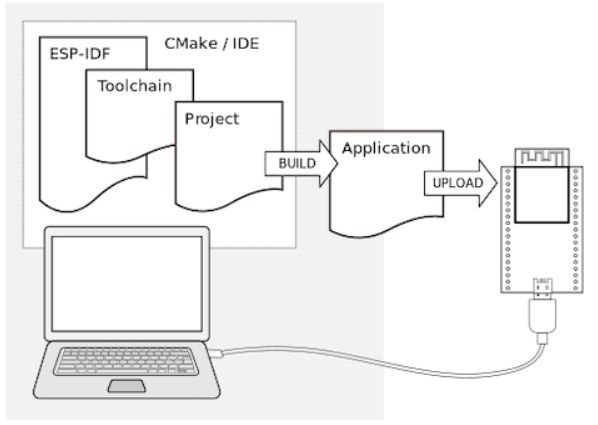
\includegraphics[width=0.5\textwidth]{images/esp-idf.png}
    \caption{ESP-IDF software flow.}
    \label{fig:espidf} % This is the image label, with which you can refer to the image in any document location.
\end{figure}

More details available on the official documentation \cite{ESP-IDF-Page}.


